\documentclass[twoside]{book}

% Packages required by doxygen
\usepackage{fixltx2e}
\usepackage{calc}
\usepackage{doxygen}
\usepackage[export]{adjustbox} % also loads graphicx
\usepackage{graphicx}
\usepackage[utf8]{inputenc}
\usepackage{makeidx}
\usepackage{multicol}
\usepackage{multirow}
\PassOptionsToPackage{warn}{textcomp}
\usepackage{textcomp}
\usepackage[nointegrals]{wasysym}
\usepackage[table]{xcolor}

% Font selection
\usepackage[T1]{fontenc}
\usepackage[scaled=.90]{helvet}
\usepackage{courier}
\usepackage{amssymb}
\usepackage{sectsty}
\renewcommand{\familydefault}{\sfdefault}
\allsectionsfont{%
  \fontseries{bc}\selectfont%
  \color{darkgray}%
}
\renewcommand{\DoxyLabelFont}{%
  \fontseries{bc}\selectfont%
  \color{darkgray}%
}
\newcommand{\+}{\discretionary{\mbox{\scriptsize$\hookleftarrow$}}{}{}}

% Page & text layout
\usepackage{geometry}
\geometry{%
  a4paper,%
  top=2.5cm,%
  bottom=2.5cm,%
  left=2.5cm,%
  right=2.5cm%
}
\tolerance=750
\hfuzz=15pt
\hbadness=750
\setlength{\emergencystretch}{15pt}
\setlength{\parindent}{0cm}
\setlength{\parskip}{3ex plus 2ex minus 2ex}
\makeatletter
\renewcommand{\paragraph}{%
  \@startsection{paragraph}{4}{0ex}{-1.0ex}{1.0ex}{%
    \normalfont\normalsize\bfseries\SS@parafont%
  }%
}
\renewcommand{\subparagraph}{%
  \@startsection{subparagraph}{5}{0ex}{-1.0ex}{1.0ex}{%
    \normalfont\normalsize\bfseries\SS@subparafont%
  }%
}
\makeatother

% Headers & footers
\usepackage{fancyhdr}
\pagestyle{fancyplain}
\fancyhead[LE]{\fancyplain{}{\bfseries\thepage}}
\fancyhead[CE]{\fancyplain{}{}}
\fancyhead[RE]{\fancyplain{}{\bfseries\leftmark}}
\fancyhead[LO]{\fancyplain{}{\bfseries\rightmark}}
\fancyhead[CO]{\fancyplain{}{}}
\fancyhead[RO]{\fancyplain{}{\bfseries\thepage}}
\fancyfoot[LE]{\fancyplain{}{}}
\fancyfoot[CE]{\fancyplain{}{}}
\fancyfoot[RE]{\fancyplain{}{\bfseries\scriptsize Generated by Doxygen }}
\fancyfoot[LO]{\fancyplain{}{\bfseries\scriptsize Generated by Doxygen }}
\fancyfoot[CO]{\fancyplain{}{}}
\fancyfoot[RO]{\fancyplain{}{}}
\renewcommand{\footrulewidth}{0.4pt}
\renewcommand{\chaptermark}[1]{%
  \markboth{#1}{}%
}
\renewcommand{\sectionmark}[1]{%
  \markright{\thesection\ #1}%
}

% Indices & bibliography
\usepackage{natbib}
\usepackage[titles]{tocloft}
\setcounter{tocdepth}{3}
\setcounter{secnumdepth}{5}
\makeindex

% Hyperlinks (required, but should be loaded last)
\usepackage{ifpdf}
\ifpdf
  \usepackage[pdftex,pagebackref=true]{hyperref}
\else
  \usepackage[ps2pdf,pagebackref=true]{hyperref}
\fi
\hypersetup{%
  colorlinks=true,%
  linkcolor=blue,%
  citecolor=blue,%
  unicode%
}

% Custom commands
\newcommand{\clearemptydoublepage}{%
  \newpage{\pagestyle{empty}\cleardoublepage}%
}

\usepackage{caption}
\captionsetup{labelsep=space,justification=centering,font={bf},singlelinecheck=off,skip=4pt,position=top}

%===== C O N T E N T S =====

\begin{document}

% Titlepage & ToC
\hypersetup{pageanchor=false,
             bookmarksnumbered=true,
             pdfencoding=unicode
            }
\pagenumbering{roman}
\begin{titlepage}
\vspace*{7cm}
\begin{center}%
{\Large Robot\+Dyn 4-\/digit display library for Arduino \\[1ex]\large 1.\+0.\+0 }\\
\vspace*{1cm}
{\large Generated by Doxygen 1.8.11}\\
\end{center}
\end{titlepage}
\clearemptydoublepage
\tableofcontents
\clearemptydoublepage
\pagenumbering{arabic}
\hypersetup{pageanchor=true}

%--- Begin generated contents ---
\chapter{Robot\+Dyn 4-\/digit L\+ED display with T\+M1637 library for Arduino.}
\label{index}\hypertarget{index}{}\href{https://travis-ci.org/Erriez/ErriezRobotDyn4DigitDisplay}{\tt }

This is a Robot\+Dyn 4-\/digit 7-\/segment L\+ED display library for Arduino. The P\+CB contains a two wire \href{https://github.com/Erriez/ErriezTM1637}{\tt T\+M1637 L\+ED / button} controller.



{\bfseries Note}\+: This library uses the double-\/dot to display a time. The L\+ED dots per segment are not wired and cannot be controlled.

\subsection*{Library features}


\begin{DoxyItemize}
\item Set brightness (0..7)
\item Set digit (0..3)
\item Control all individual segments per digit
\item Control double dots (on/off)
\item Display time (hours\+:minutes)
\item Display decimal value (-\/999..9999) with optional padding
\item Display hexadecimal value (0...0x\+F\+F\+FF) with optional padding
\end{DoxyItemize}

\subsection*{Hardware}

{\bfseries Connection display with Arduino}

\tabulinesep=1mm
\begin{longtabu} spread 0pt [c]{*2{|X[-1]}|}
\hline
\rowcolor{\tableheadbgcolor}\PBS\centering {\bf Display }&{\bf Arduino U\+NO / Nano / Pro Mini / Leonardo / Mega2560 / E\+S\+P8266 / Lolin32  }\\\cline{1-2}
\endfirsthead
\hline
\endfoot
\hline
\rowcolor{\tableheadbgcolor}\PBS\centering {\bf Display }&{\bf Arduino U\+NO / Nano / Pro Mini / Leonardo / Mega2560 / E\+S\+P8266 / Lolin32  }\\\cline{1-2}
\endhead
\PBS\centering G\+ND &G\+ND \\\cline{1-2}
\PBS\centering V\+CC &5V (or 3.\+3V) \\\cline{1-2}
\PBS\centering C\+LK &Any D\+I\+G\+I\+T\+AL pin \\\cline{1-2}
\PBS\centering D\+IO &Any D\+I\+G\+I\+T\+AL pin \\\cline{1-2}
\end{longtabu}
Other M\+CU\textquotesingle{}s may work, but are not tested.

\subsection*{Examples}

Examples $\vert$ Erriez Robot\+Dyn 4-\/digit display $\vert$ \href{https://github.com/Erriez/ErriezRobotDyn4DigitDisplay/blob/master/examples/7SegementDisplayDemo/7SegementDisplayDemo.ino}{\tt 7\+Segement\+Display\+Demo}

\subsection*{Documentation}


\begin{DoxyItemize}
\item \href{https://erriez.github.io/ErriezRobotDyn4DigitDisplay}{\tt Online H\+T\+ML}
\item \href{https://github.com/Erriez/ErriezRobotDyn4DigitDisplay/raw/gh-pages/latex/ErriezRobotDyn4DigitDisplay.pdf}{\tt Download P\+DF}
\end{DoxyItemize}

\subsection*{Usage}

{\bfseries Initialization}


\begin{DoxyCode}
1 \{c++\}
2 #include <RobotDyn4DigitDisplay.h>
3 
4 // Connect display pins to the Arduino DIGITAL pins
5 #if defined(ARDUINO\_ARCH\_AVR)
6 #define TM1637\_CLK\_PIN      2
7 #define TM1637\_DIO\_PIN      3
8 #elif defined(ARDUINO\_ESP8266\_WEMOS\_D1MINI) || defined(ESP8266\_WEMOS\_D1MINI) ||
       defined(ARDUINO\_ESP8266\_NODEMCU)
9 #define TM1637\_CLK\_PIN      D2
10 #define TM1637\_DIO\_PIN      D3
11 #elif defined(ARDUINO\_LOLIN32)
12 #define TM1637\_CLK\_PIN      0
13 #define TM1637\_DIO\_PIN      4
14 #else
15 #error "May work, but not tested on this target"
16 #endif
17 
18 // Create display object
19 RobotDyn4DigitDisplay display(TM1637\_CLK\_PIN, TM1637\_DIO\_PIN);
20 
21 void setup()
22 \{
23     // Initialize TM1637
24     display.begin();
25 \}
\end{DoxyCode}


{\bfseries Clear display}


\begin{DoxyCode}
1 \{c++\}
2 // Clear display
3 display.clear();    // \_ \_ \_ \_
\end{DoxyCode}


{\bfseries Set brightness}


\begin{DoxyCode}
1 \{c++\}
2 // Set brightness
3 display.setBrightness(0); // Minimum
4 display.setBrightness(7); // Maximum
\end{DoxyCode}


{\bfseries Display time}


\begin{DoxyCode}
1 \{c++\}
2 // Display time
3 display.time(11, 59);   // 1 1 : 5 9
\end{DoxyCode}


{\bfseries Control time double dot}


\begin{DoxyCode}
1 \{c++\}
2 display.doubleDots(true);   // Turn double dot on
3 display.doubleDots(false);  // Turn double dot off
\end{DoxyCode}


{\bfseries Display decimal value}


\begin{DoxyCode}
1 \{c++\}
2 // Display decimal values
3 display.dec(-999);  // - 9 9 9
4 display.dec(-1);    // \_ \_ - 1
5 display.dec(0);     // \_ \_ \_ 0
6 display.dec(1);     // \_ \_ \_ 1
7 display.dec(123);   // \_ 1 2 3
8 display.dec(9999);  // 9 9 9 9
9 display.dec(10000); // - - - -
10 
11 // Display decimal values with padding
12 display.dec(1);     // \_ \_ \_ 1  (Default no padding)
13 display.dec(1, 2);  // \_ \_ 0 1  (2 digits padding)
14 display.dec(1, 3);  // \_ 0 0 1  (3 digits padding)
15 display.dec(1, 4);  // 0 0 0 1  (4 digits padding)
16 
17 display.dec(34, 3); // \_ 0 3 4  (2 digits padding)
\end{DoxyCode}


{\bfseries Display hexadecimal value}


\begin{DoxyCode}
1 \{c++\}
2 // Display hexadecimal values
3 display.dec(0x0000);    // 0 0 0 0
4 display.dec(0x1234);    // 1 2 3 4
5 display.dec(0xABCD);    // A B C D
6 display.dec(0xBEEF);    // B E E F
7 
8 // Display hexadecimal values with padding
9 display.hex(0x0001);    // \_ \_ \_ 1  (Default no padding)
10 display.hex(0x0001, 2); // \_ \_ 0 1  (2 digits padding)
11 display.hex(0x0001, 3); // \_ 0 0 1  (3 digits padding)
12 display.hex(0x0001, 4); // 0 0 0 1  (4 digits padding)
13 
14 display.hex(0x0034, 3); // \_ 0 3 4  (2 digits padding)
\end{DoxyCode}


{\bfseries Control individual digits}


\begin{DoxyCode}
1 \{c++\}
2 // Display individual digits: 1 2 3 4
3 display.digit(0, 1);
4 display.digit(1, 2);
5 display.digit(2, 3);
6 display.digit(3, 4);
\end{DoxyCode}


{\bfseries Special characters}


\begin{DoxyCode}
1 \{c++\}
2 Control individual LED-segments (bit numbers):
3    - 0 -
4    |   |
5    5   1
6    |   |
7    - 6 -
8    |   |
9    4   2
10    |   |
11    - 3 -  .7
12 
13 // Display error: E r r \_
14 display.rawDigit(0, 0b01111001);
15 display.rawDigit(1, 0b01010000);
16 display.rawDigit(2, 0b01010000);
17 display.rawDigit(3, 0b00000000);
18 
19 // Display H character: \_ \_ \_ H
20 display.rawDigit(3, 0b01110110);
21 
22 // Display negative temperature: - 1 ` C
23 display.rawDigit(0, SEGMENTS\_MINUS);
24 display.digit(1, 1);
25 display.rawDigit(2, SEGMENTS\_DEGREE);
26 display.rawDigit(3, SEGMENTS\_CELSIUS);
27 
28 // Display rect
29 display.rawDigit(0, 0b00111001);
30 display.rawDigit(1, 0b00001001);
31 display.rawDigit(2, 0b00001001);
32 display.rawDigit(3, 0b00001111);
\end{DoxyCode}


\subsection*{Library dependencies}


\begin{DoxyItemize}
\item \href{https://github.com/Erriez/ErriezTM1637}{\tt Erriez T\+M1637} library
\end{DoxyItemize}

\subsection*{Library installation}

Please refer to the \href{https://github.com/Erriez/ErriezArduinoLibrariesAndSketches/wiki}{\tt Wiki} page.

\subsection*{Other Arduino Libraries and Sketches from Erriez}


\begin{DoxyItemize}
\item \href{https://github.com/Erriez/ErriezArduinoLibrariesAndSketches}{\tt Erriez Libraries and Sketches} 
\end{DoxyItemize}
\chapter{Hierarchical Index}
\section{Class Hierarchy}
This inheritance list is sorted roughly, but not completely, alphabetically\+:\begin{DoxyCompactList}
\item T\+M1637\begin{DoxyCompactList}
\item \contentsline{section}{Robot\+Dyn4\+Digit\+Display}{\pageref{class_robot_dyn4_digit_display}}{}
\end{DoxyCompactList}
\end{DoxyCompactList}

\chapter{Class Index}
\section{Class List}
Here are the classes, structs, unions and interfaces with brief descriptions\+:\begin{DoxyCompactList}
\item\contentsline{section}{\hyperlink{class_robot_dyn4_digit_display}{Robot\+Dyn4\+Digit\+Display} \\*\hyperlink{class_robot_dyn4_digit_display}{Robot\+Dyn4\+Digit\+Display} class }{\pageref{class_robot_dyn4_digit_display}}{}
\end{DoxyCompactList}

\chapter{File Index}
\section{File List}
Here is a list of all documented files with brief descriptions\+:\begin{DoxyCompactList}
\item\contentsline{section}{\hyperlink{_robot_dyn4_digit_display_8cpp}{Robot\+Dyn4\+Digit\+Display.\+cpp} \\*\hyperlink{class_robot_dyn4_digit_display}{Robot\+Dyn4\+Digit\+Display} library for Arduino }{\pageref{_robot_dyn4_digit_display_8cpp}}{}
\item\contentsline{section}{\hyperlink{_robot_dyn4_digit_display_8h}{Robot\+Dyn4\+Digit\+Display.\+h} \\*\hyperlink{class_robot_dyn4_digit_display}{Robot\+Dyn4\+Digit\+Display} library for Arduino }{\pageref{_robot_dyn4_digit_display_8h}}{}
\end{DoxyCompactList}

\chapter{Class Documentation}
\hypertarget{class_robot_dyn4_digit_display}{}\section{Robot\+Dyn4\+Digit\+Display Class Reference}
\label{class_robot_dyn4_digit_display}\index{Robot\+Dyn4\+Digit\+Display@{Robot\+Dyn4\+Digit\+Display}}


\hyperlink{class_robot_dyn4_digit_display}{Robot\+Dyn4\+Digit\+Display} class.  




{\ttfamily \#include $<$Robot\+Dyn4\+Digit\+Display.\+h$>$}

Inheritance diagram for Robot\+Dyn4\+Digit\+Display\+:\begin{figure}[H]
\begin{center}
\leavevmode
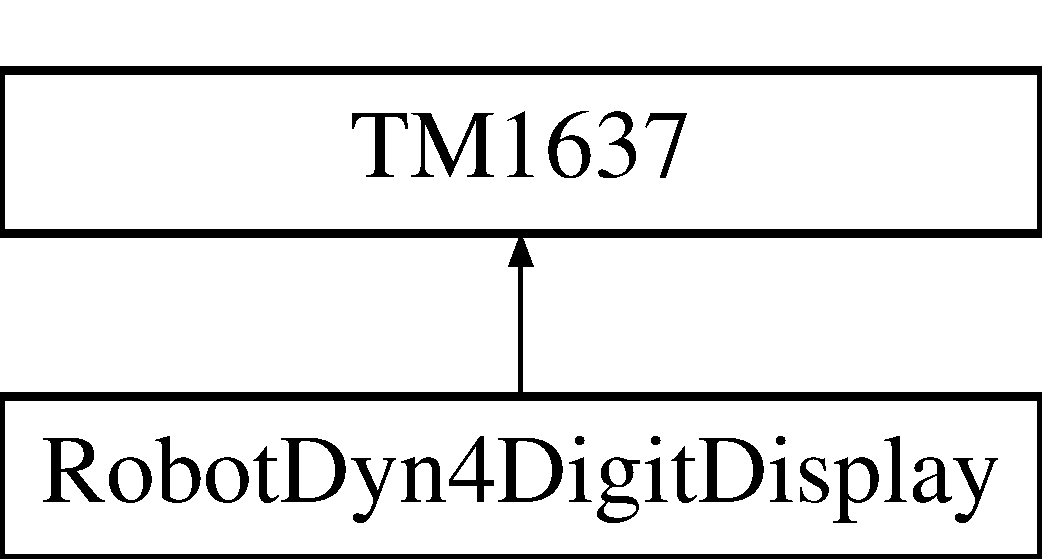
\includegraphics[height=2.000000cm]{class_robot_dyn4_digit_display}
\end{center}
\end{figure}
\subsection*{Public Member Functions}
\begin{DoxyCompactItemize}
\item 
\hyperlink{class_robot_dyn4_digit_display_ad4240ac103a42b221593fb0110aa8032}{Robot\+Dyn4\+Digit\+Display} (uint8\+\_\+t clk\+Pin, uint8\+\_\+t dio\+Pin, bool display\+On=true, uint8\+\_\+t brightness=5)
\begin{DoxyCompactList}\small\item\em Constructor Robot\+Dyn 4-\/digit L\+ED display. \end{DoxyCompactList}\item 
void \hyperlink{class_robot_dyn4_digit_display_a7f990760be0a939de2e97c323f93e91a}{raw\+Digit} (uint8\+\_\+t \hyperlink{class_robot_dyn4_digit_display_aa0a682be1d560c1c93f547539b971806}{digit}, uint8\+\_\+t value)
\begin{DoxyCompactList}\small\item\em Display raw digit. \end{DoxyCompactList}\item 
void \hyperlink{class_robot_dyn4_digit_display_aa0a682be1d560c1c93f547539b971806}{digit} (uint8\+\_\+t digit, uint8\+\_\+t value)
\begin{DoxyCompactList}\small\item\em Display a single digit. \end{DoxyCompactList}\item 
void \hyperlink{class_robot_dyn4_digit_display_a1906505c29cfcb7baa7f4b9162301f6e}{double\+Dots} (bool on)
\begin{DoxyCompactList}\small\item\em Display double time dots. \end{DoxyCompactList}\item 
void \hyperlink{class_robot_dyn4_digit_display_aa7382284633fff676ae746f0270024bd}{time} (uint8\+\_\+t hour, uint8\+\_\+t minute, bool double\+Dots\+On=true, bool pad\+Hours=true)
\begin{DoxyCompactList}\small\item\em Display time. \end{DoxyCompactList}\item 
void \hyperlink{class_robot_dyn4_digit_display_af99a7b39a0e4dc6bfa8d1fef6a835651}{dec} (int value, uint8\+\_\+t pad=1)
\begin{DoxyCompactList}\small\item\em Display decimal value. \end{DoxyCompactList}\item 
void \hyperlink{class_robot_dyn4_digit_display_a3f1e8418ba6d4b3be5a10296213f099f}{hex} (unsigned int value, uint8\+\_\+t pad=4)
\begin{DoxyCompactList}\small\item\em Display hexadecimal value with optional padding. \end{DoxyCompactList}\item 
void \hyperlink{class_robot_dyn4_digit_display_a3b7b4da4d448c85358f5dad20cd1dbd6}{overflow} ()\hypertarget{class_robot_dyn4_digit_display_a3b7b4da4d448c85358f5dad20cd1dbd6}{}\label{class_robot_dyn4_digit_display_a3b7b4da4d448c85358f5dad20cd1dbd6}

\begin{DoxyCompactList}\small\item\em Display overflow with four minus digits. \end{DoxyCompactList}\end{DoxyCompactItemize}


\subsection{Detailed Description}
\hyperlink{class_robot_dyn4_digit_display}{Robot\+Dyn4\+Digit\+Display} class. 

This class 

Definition at line 52 of file Robot\+Dyn4\+Digit\+Display.\+h.



\subsection{Constructor \& Destructor Documentation}
\index{Robot\+Dyn4\+Digit\+Display@{Robot\+Dyn4\+Digit\+Display}!Robot\+Dyn4\+Digit\+Display@{Robot\+Dyn4\+Digit\+Display}}
\index{Robot\+Dyn4\+Digit\+Display@{Robot\+Dyn4\+Digit\+Display}!Robot\+Dyn4\+Digit\+Display@{Robot\+Dyn4\+Digit\+Display}}
\subsubsection[{\texorpdfstring{Robot\+Dyn4\+Digit\+Display(uint8\+\_\+t clk\+Pin, uint8\+\_\+t dio\+Pin, bool display\+On=true, uint8\+\_\+t brightness=5)}{RobotDyn4DigitDisplay(uint8_t clkPin, uint8_t dioPin, bool displayOn=true, uint8_t brightness=5)}}]{\setlength{\rightskip}{0pt plus 5cm}Robot\+Dyn4\+Digit\+Display\+::\+Robot\+Dyn4\+Digit\+Display (
\begin{DoxyParamCaption}
\item[{uint8\+\_\+t}]{clk\+Pin, }
\item[{uint8\+\_\+t}]{dio\+Pin, }
\item[{bool}]{display\+On = {\ttfamily true}, }
\item[{uint8\+\_\+t}]{brightness = {\ttfamily 5}}
\end{DoxyParamCaption}
)}\hypertarget{class_robot_dyn4_digit_display_ad4240ac103a42b221593fb0110aa8032}{}\label{class_robot_dyn4_digit_display_ad4240ac103a42b221593fb0110aa8032}


Constructor Robot\+Dyn 4-\/digit L\+ED display. 


\begin{DoxyParams}{Parameters}
{\em clk\+Pin} & Clock pins. \\
\hline
{\em dio\+Pin} & Bi-\/directional data pin. \\
\hline
{\em display\+On} & Optional\+: Turn display on. Default\+: true \\
\hline
{\em brightness} & Optional\+: Set brightness 0..7 Default\+: 5. \\
\hline
\end{DoxyParams}


Definition at line 84 of file Robot\+Dyn4\+Digit\+Display.\+cpp.



\subsection{Member Function Documentation}
\index{Robot\+Dyn4\+Digit\+Display@{Robot\+Dyn4\+Digit\+Display}!dec@{dec}}
\index{dec@{dec}!Robot\+Dyn4\+Digit\+Display@{Robot\+Dyn4\+Digit\+Display}}
\subsubsection[{\texorpdfstring{dec(int value, uint8\+\_\+t pad=1)}{dec(int value, uint8_t pad=1)}}]{\setlength{\rightskip}{0pt plus 5cm}void Robot\+Dyn4\+Digit\+Display\+::dec (
\begin{DoxyParamCaption}
\item[{int}]{value, }
\item[{uint8\+\_\+t}]{pad = {\ttfamily 1}}
\end{DoxyParamCaption}
)}\hypertarget{class_robot_dyn4_digit_display_af99a7b39a0e4dc6bfa8d1fef6a835651}{}\label{class_robot_dyn4_digit_display_af99a7b39a0e4dc6bfa8d1fef6a835651}


Display decimal value. 


\begin{DoxyParams}{Parameters}
{\em value} & 0000..9999\+: Decimal value. \\
\hline
{\em pad} & 0..4\+: Optional\+: Number of digits to pad with a zero. Default\+: 1. \\
\hline
\end{DoxyParams}


Definition at line 170 of file Robot\+Dyn4\+Digit\+Display.\+cpp.

\index{Robot\+Dyn4\+Digit\+Display@{Robot\+Dyn4\+Digit\+Display}!digit@{digit}}
\index{digit@{digit}!Robot\+Dyn4\+Digit\+Display@{Robot\+Dyn4\+Digit\+Display}}
\subsubsection[{\texorpdfstring{digit(uint8\+\_\+t digit, uint8\+\_\+t value)}{digit(uint8_t digit, uint8_t value)}}]{\setlength{\rightskip}{0pt plus 5cm}void Robot\+Dyn4\+Digit\+Display\+::digit (
\begin{DoxyParamCaption}
\item[{uint8\+\_\+t}]{digit, }
\item[{uint8\+\_\+t}]{value}
\end{DoxyParamCaption}
)}\hypertarget{class_robot_dyn4_digit_display_aa0a682be1d560c1c93f547539b971806}{}\label{class_robot_dyn4_digit_display_aa0a682be1d560c1c93f547539b971806}


Display a single digit. 


\begin{DoxyParams}{Parameters}
{\em digit} & Digit number 0 (left digit) ... 3 (right digit) \\
\hline
{\em value} & Digit value 0..9 or 0x00..0x0F. \\
\hline
\end{DoxyParams}


Definition at line 113 of file Robot\+Dyn4\+Digit\+Display.\+cpp.

\index{Robot\+Dyn4\+Digit\+Display@{Robot\+Dyn4\+Digit\+Display}!double\+Dots@{double\+Dots}}
\index{double\+Dots@{double\+Dots}!Robot\+Dyn4\+Digit\+Display@{Robot\+Dyn4\+Digit\+Display}}
\subsubsection[{\texorpdfstring{double\+Dots(bool on)}{doubleDots(bool on)}}]{\setlength{\rightskip}{0pt plus 5cm}void Robot\+Dyn4\+Digit\+Display\+::double\+Dots (
\begin{DoxyParamCaption}
\item[{bool}]{on}
\end{DoxyParamCaption}
)}\hypertarget{class_robot_dyn4_digit_display_a1906505c29cfcb7baa7f4b9162301f6e}{}\label{class_robot_dyn4_digit_display_a1906505c29cfcb7baa7f4b9162301f6e}


Display double time dots. 


\begin{DoxyParams}{Parameters}
{\em on} & true\+: Turn double time dots on.~\newline
 false\+: Turn double time dots off. \\
\hline
\end{DoxyParams}


Definition at line 126 of file Robot\+Dyn4\+Digit\+Display.\+cpp.

\index{Robot\+Dyn4\+Digit\+Display@{Robot\+Dyn4\+Digit\+Display}!hex@{hex}}
\index{hex@{hex}!Robot\+Dyn4\+Digit\+Display@{Robot\+Dyn4\+Digit\+Display}}
\subsubsection[{\texorpdfstring{hex(unsigned int value, uint8\+\_\+t pad=4)}{hex(unsigned int value, uint8_t pad=4)}}]{\setlength{\rightskip}{0pt plus 5cm}void Robot\+Dyn4\+Digit\+Display\+::hex (
\begin{DoxyParamCaption}
\item[{unsigned int}]{value, }
\item[{uint8\+\_\+t}]{pad = {\ttfamily 4}}
\end{DoxyParamCaption}
)}\hypertarget{class_robot_dyn4_digit_display_a3f1e8418ba6d4b3be5a10296213f099f}{}\label{class_robot_dyn4_digit_display_a3f1e8418ba6d4b3be5a10296213f099f}


Display hexadecimal value with optional padding. 


\begin{DoxyParams}{Parameters}
{\em value} & 0x0000..0x\+F\+F\+FF\+: Hexadecimal value \\
\hline
{\em pad} & 0..4\+: Optional\+: Number of digits to pad with a zero. Default\+: 4. \\
\hline
\end{DoxyParams}


Definition at line 224 of file Robot\+Dyn4\+Digit\+Display.\+cpp.

\index{Robot\+Dyn4\+Digit\+Display@{Robot\+Dyn4\+Digit\+Display}!raw\+Digit@{raw\+Digit}}
\index{raw\+Digit@{raw\+Digit}!Robot\+Dyn4\+Digit\+Display@{Robot\+Dyn4\+Digit\+Display}}
\subsubsection[{\texorpdfstring{raw\+Digit(uint8\+\_\+t digit, uint8\+\_\+t value)}{rawDigit(uint8_t digit, uint8_t value)}}]{\setlength{\rightskip}{0pt plus 5cm}void Robot\+Dyn4\+Digit\+Display\+::raw\+Digit (
\begin{DoxyParamCaption}
\item[{uint8\+\_\+t}]{digit, }
\item[{uint8\+\_\+t}]{value}
\end{DoxyParamCaption}
)}\hypertarget{class_robot_dyn4_digit_display_a7f990760be0a939de2e97c323f93e91a}{}\label{class_robot_dyn4_digit_display_a7f990760be0a939de2e97c323f93e91a}


Display raw digit. 


\begin{DoxyParams}{Parameters}
{\em digit} & Digit number 0 (left digit) .. 3 (right digit) \\
\hline
{\em value} & L\+ED segments \\
\hline
\end{DoxyParams}


Definition at line 98 of file Robot\+Dyn4\+Digit\+Display.\+cpp.

\index{Robot\+Dyn4\+Digit\+Display@{Robot\+Dyn4\+Digit\+Display}!time@{time}}
\index{time@{time}!Robot\+Dyn4\+Digit\+Display@{Robot\+Dyn4\+Digit\+Display}}
\subsubsection[{\texorpdfstring{time(uint8\+\_\+t hour, uint8\+\_\+t minute, bool double\+Dots\+On=true, bool pad\+Hours=true)}{time(uint8_t hour, uint8_t minute, bool doubleDotsOn=true, bool padHours=true)}}]{\setlength{\rightskip}{0pt plus 5cm}void Robot\+Dyn4\+Digit\+Display\+::time (
\begin{DoxyParamCaption}
\item[{uint8\+\_\+t}]{hour, }
\item[{uint8\+\_\+t}]{minute, }
\item[{bool}]{double\+Dots\+On = {\ttfamily true}, }
\item[{bool}]{pad\+Hours = {\ttfamily true}}
\end{DoxyParamCaption}
)}\hypertarget{class_robot_dyn4_digit_display_aa7382284633fff676ae746f0270024bd}{}\label{class_robot_dyn4_digit_display_aa7382284633fff676ae746f0270024bd}


Display time. 


\begin{DoxyParams}{Parameters}
{\em hour} & 0..59\+: Hours \\
\hline
{\em minute} & 0..59\+: Minutes \\
\hline
{\em double\+Dots\+On} & true\+: Display double time dots. (Default)~\newline
 false\+: Turn double time dots off. \\
\hline
{\em pad\+Hours} & true\+: Display first digit as 0 when hours $<$ 10. false\+: Turn first digit off when hours $<$ 10. \\
\hline
\end{DoxyParams}


Definition at line 149 of file Robot\+Dyn4\+Digit\+Display.\+cpp.



The documentation for this class was generated from the following files\+:\begin{DoxyCompactItemize}
\item 
\hyperlink{_robot_dyn4_digit_display_8h}{Robot\+Dyn4\+Digit\+Display.\+h}\item 
\hyperlink{_robot_dyn4_digit_display_8cpp}{Robot\+Dyn4\+Digit\+Display.\+cpp}\end{DoxyCompactItemize}

\chapter{File Documentation}
\hypertarget{_robot_dyn4_digit_display_8cpp}{}\section{Robot\+Dyn4\+Digit\+Display.\+cpp File Reference}
\label{_robot_dyn4_digit_display_8cpp}\index{Robot\+Dyn4\+Digit\+Display.\+cpp@{Robot\+Dyn4\+Digit\+Display.\+cpp}}


\hyperlink{class_robot_dyn4_digit_display}{Robot\+Dyn4\+Digit\+Display} library for Arduino.  


{\ttfamily \#include $<$pgmspace.\+h$>$}\\*
{\ttfamily \#include \char`\"{}Robot\+Dyn4\+Digit\+Display.\+h\char`\"{}}\\*


\subsection{Detailed Description}
\hyperlink{class_robot_dyn4_digit_display}{Robot\+Dyn4\+Digit\+Display} library for Arduino. 

Source\+: \href{https://github.com/Erriez/ErriezRobotDyn4DigitDisplay}{\tt https\+://github.\+com/\+Erriez/\+Erriez\+Robot\+Dyn4\+Digit\+Display} Documentation\+: \href{https://erriez.github.io/ErriezRobotDyn4DigitDisplay}{\tt https\+://erriez.\+github.\+io/\+Erriez\+Robot\+Dyn4\+Digit\+Display} 
\hypertarget{_robot_dyn4_digit_display_8h}{}\section{Robot\+Dyn4\+Digit\+Display.\+h File Reference}
\label{_robot_dyn4_digit_display_8h}\index{Robot\+Dyn4\+Digit\+Display.\+h@{Robot\+Dyn4\+Digit\+Display.\+h}}


\hyperlink{class_robot_dyn4_digit_display}{Robot\+Dyn4\+Digit\+Display} library for Arduino.  


{\ttfamily \#include $<$Arduino.\+h$>$}\\*
{\ttfamily \#include $<$T\+M1637.\+h$>$}\\*
\subsection*{Classes}
\begin{DoxyCompactItemize}
\item 
class \hyperlink{class_robot_dyn4_digit_display}{Robot\+Dyn4\+Digit\+Display}
\begin{DoxyCompactList}\small\item\em \hyperlink{class_robot_dyn4_digit_display}{Robot\+Dyn4\+Digit\+Display} class. \end{DoxyCompactList}\end{DoxyCompactItemize}
\subsection*{Macros}
\begin{DoxyCompactItemize}
\item 
\#define \hyperlink{_robot_dyn4_digit_display_8h_a9b7ce6f9f8b0b718863bbb3a925c274f}{R\+O\+B\+O\+T\+\_\+\+D\+Y\+N\+\_\+4\+D\+I\+G\+I\+T\+\_\+\+D\+I\+S\+P\+L\+A\+Y\+\_\+\+N\+U\+M\+\_\+\+D\+I\+G\+I\+TS}~4\hypertarget{_robot_dyn4_digit_display_8h_a9b7ce6f9f8b0b718863bbb3a925c274f}{}\label{_robot_dyn4_digit_display_8h_a9b7ce6f9f8b0b718863bbb3a925c274f}

\begin{DoxyCompactList}\small\item\em Number of display digits. \end{DoxyCompactList}\item 
\#define \hyperlink{_robot_dyn4_digit_display_8h_aebe5e8b346e8ecec5f95302cb6acef1c}{S\+E\+G\+M\+E\+N\+T\+S\+\_\+\+M\+I\+N\+US}~0b01000000
\begin{DoxyCompactList}\small\item\em Special characters. \end{DoxyCompactList}\item 
\#define \hyperlink{_robot_dyn4_digit_display_8h_a4d8b2aa23a47869894c401c2d1345750}{S\+E\+G\+M\+E\+N\+T\+S\+\_\+\+D\+E\+G\+R\+EE}~0b01100011\hypertarget{_robot_dyn4_digit_display_8h_a4d8b2aa23a47869894c401c2d1345750}{}\label{_robot_dyn4_digit_display_8h_a4d8b2aa23a47869894c401c2d1345750}

\begin{DoxyCompactList}\small\item\em Degree symbol. \end{DoxyCompactList}\item 
\#define \hyperlink{_robot_dyn4_digit_display_8h_a0e80a13de7d7002a4e6d9124db9a2d15}{S\+E\+G\+M\+E\+N\+T\+S\+\_\+\+C\+E\+L\+S\+I\+US}~0b00111001\hypertarget{_robot_dyn4_digit_display_8h_a0e80a13de7d7002a4e6d9124db9a2d15}{}\label{_robot_dyn4_digit_display_8h_a0e80a13de7d7002a4e6d9124db9a2d15}

\begin{DoxyCompactList}\small\item\em Celsius symbol. \end{DoxyCompactList}\end{DoxyCompactItemize}


\subsection{Detailed Description}
\hyperlink{class_robot_dyn4_digit_display}{Robot\+Dyn4\+Digit\+Display} library for Arduino. 

Source\+: \href{https://github.com/Erriez/ErriezRobotDyn4DigitDisplay}{\tt https\+://github.\+com/\+Erriez/\+Erriez\+Robot\+Dyn4\+Digit\+Display} Documentation\+: \href{https://erriez.github.io/ErriezRobotDyn4DigitDisplay}{\tt https\+://erriez.\+github.\+io/\+Erriez\+Robot\+Dyn4\+Digit\+Display} 

\subsection{Macro Definition Documentation}
\index{Robot\+Dyn4\+Digit\+Display.\+h@{Robot\+Dyn4\+Digit\+Display.\+h}!S\+E\+G\+M\+E\+N\+T\+S\+\_\+\+M\+I\+N\+US@{S\+E\+G\+M\+E\+N\+T\+S\+\_\+\+M\+I\+N\+US}}
\index{S\+E\+G\+M\+E\+N\+T\+S\+\_\+\+M\+I\+N\+US@{S\+E\+G\+M\+E\+N\+T\+S\+\_\+\+M\+I\+N\+US}!Robot\+Dyn4\+Digit\+Display.\+h@{Robot\+Dyn4\+Digit\+Display.\+h}}
\subsubsection[{\texorpdfstring{S\+E\+G\+M\+E\+N\+T\+S\+\_\+\+M\+I\+N\+US}{SEGMENTS_MINUS}}]{\setlength{\rightskip}{0pt plus 5cm}\#define S\+E\+G\+M\+E\+N\+T\+S\+\_\+\+M\+I\+N\+US~0b01000000}\hypertarget{_robot_dyn4_digit_display_8h_aebe5e8b346e8ecec5f95302cb6acef1c}{}\label{_robot_dyn4_digit_display_8h_aebe5e8b346e8ecec5f95302cb6acef1c}


Special characters. 

Minus sign 

Definition at line 43 of file Robot\+Dyn4\+Digit\+Display.\+h.


%--- End generated contents ---

% Index
\backmatter
\newpage
\phantomsection
\clearemptydoublepage
\addcontentsline{toc}{chapter}{Index}
\printindex

\end{document}
